\documentclass[a4paper, 12pt]{article}
\usepackage[utf8]{inputenc}%%seul package à charger~: pour éviter les problèmes sordides d'encodage
\usepackage[rapport, psc]{andre}%%bon eh bien sûr...

\usepackage{makeidx}              %% permet de générer un index automatiquement
\usepackage[style=numeric, backend=bibtex]{biblatex}				%% Utilisé pour la biblio
\usepackage[hidelinks]{hyperref}
\usepackage{graphicx}



\title{Projet Scientifique Collectif X2013 \\INF02~: Synthétiseur automatique de documents \\Rapport final}
\renewcommand{\petittitre}{Projet INF02}
\newcommand{\pyt}[1]{\texttt{#1}}%noms python
\newcommand{\ang}[1]{\textit{#1}}%noms anglais
\author{\membres} %%\membres uniquement avec l'option psc
\date{20 avril 2015}


\index{Réseau sémantique}
\index{Analyse symbolique}
\index{Analyse sémantique}
\index{Réseau de Concepts}

\makeindex
\addbibresource{biblio.bib}

\begin{document}

\titrelong{}


\tableofcontents
\newpage

\section{Rappel du projet}

\subsection{Notre groupe}
\begin{itemize}
 \item Fernandes-Pinto-Fachada Sarah, \textbf{8\textsuperscript{e}} compagnie, section \textbf{équitation};
 \item Schrottenloher André, \textbf{8\textsuperscript{e}} compagnie, section \textbf{escrime};
 \item Angibault Antonin, \textbf{8\textsuperscript{e}} compagnie, section \textbf{escrime};
 \item Hufschmitt Théophane, \textbf{8\textsuperscript{e}} compagnie, section \textbf{escrime};
 \item Cao Zhixing, \textbf{9\textsuperscript{e}} compagnie, section \textbf{escalade};
 \item Boisseau Guillaume, \textbf{6\textsuperscript{e}} compagnie, section \textbf{natation};
\end{itemize}

\subsection{Notre sujet}

\subsubsection{But du projet}
%reprise textuelle

%%reprise
Nous vivons dans un \^{a}ge d'abondance d'information, qu'il convient de traiter efficacement pour en profiter. Dans ce contexte, les synthétiseurs automatiques de textes ont bénéficié d'efforts croissants de recherche au cours des années passées. Notre travail s'inscrit dans cette démarche.

%%reprise
Un nombre non négligeable d'outils reposent, essentiellement, sur une extraction des phrases pertinentes \textit{via} une analyse statistique et éventuellement une analyse symbolique plus ou moins poussée (\textit{extractive summarization}\index{Extractive summarization}). Nous voulions mettre l'accent sur cette analyse de façon à donner une réelle compréhension des corpus à notre programme et, pour se convaincre de son succès, le pousser à la reformulation (\textit{abstractive summarization})\index{Abstractive summarization}.


Le but de notre projet était de produire un programme capable d'analyser sémantiquement\index{Analyse sémantique} un texte ayant pour sujet le sport (et plus particulièrement encore le football) de façon à en produire un résumé. Il s'agit là d'une véritable innovation par rapport à l'état actuel du résumé automatique, dans la mesure où les programmes existants se basent prioritairement sur une analyse statistique plus ou moins poussée de fréquence d'apparition des mots pour juger de leur importance~; notre programme s'appuierait plutôt sur le sens pour juger de la pertinence d'un concept et savoir s'il doit le faire figurer ou non dans le résumé final.


\subsubsection{Modules du projet et répartition du travail}
%%reprise textuelle

Pour atteindre cet objectif, plusieurs modules assez indépendants ont pu être identifiés et traités séparément~:

\begin{description}
	\item[Récupération de données] à utiliser pour la création d'un réseau de concepts modélisant la connaissance \textit{a priori} du programme. Responsables~: Théophane Hufschmitt, Guillaume Boisseau.
	\item[Création du réseau de concepts] et remplissage de celui-ci. Il s'agissait ici d'une part de définir sa structure et d'autre part d'y introduire les données nécessaires. Responsables~: André Schrottenloher, Guillaume Boisseau.
	\item[Analyse syntaxique] à l'aide d'outils existants. Il s'agissait de trouver une grammaire capable d'analyser une phrase et d'en faire ressortir les relations de type verbe-objet ou nom-qualificatif. Responsables~: Antonin Angibault, Théophane Hufschmitt, Sarah Fernandes-Pinto-Fachada.
	\item[Réflexion] sur l'utilisation du réseau de concepts et de l'analyse grammaticale pour produire un réseau capable de rendre compte de la compréhension du texte. Responsables~: tous.
	\item[Implémentation] d'un algorithme simple de résumé statistique (basé sur l'algorithme TF-IDF), devant servir de base de comparaison pour tester la qualité des résumés produits par notre algorithme.  Responsable~: Zhixing Cao.
\end{description}

\subsubsection{Outils extérieurs utilisés}

Nous reviendrons sur ces outils et détaillerons au fur et à mesure du rapport.

\begin{itemize}
	\item[WordNet~: ]Dictionnaire permettant d'obtenir la classe grammaticale des mots présents dans le réseau.
	\item[Conceptnet~: ]Grande base de connaissances permettant d'établir la proximité conceptuelle entre différents termes du réseau.
	\item[Freebase~: ]Cette base de connaissances très étendue permet d'identifier les noms propres, par exemple des joueurs de football ou différents stades.
	\item[Natural Language ToolKit (\pyt{nltk})~: ]Divers outils grammaticaux pour l'étude du langage naturel.
	\item Un analyseur syntaxique dont les résultats nous ont été fournis par Systran.
\end{itemize}


\section{État de l'art} %Revue et analyse de l’état de l’art / des approches concurrentes ou alternatives
%%%%%%%%%%%%%%%%%%%%%ù
%% WARNING : REPRISE TEXTUELLE
%%%%%%%%%%%%%%%%%%%%%%

D'après~\cite{jones_automatic_2007}, des recherches sur la synthèse automatique de documents se sont principalement développées depuis les années 1990, motivées par des analyses statistiques remontant aussi loin que 1958. Les méthodes d'extraction, de par la simplicité de leur mise en œuvre, ont été le plus mises en avant, utilisant dans des travaux plus récents une analyse symbolique plus poussée, menant à la reformulation de la source plut\^{o}t que de la simple extraction de son contenu (on parle alors d'abstraction). Dans cette section, nous détaillerons les techniques propres à ces deux paradigmes, puis nous indiquerons les méthodes envisageables d'évaluation de la qualité des résumés produits.

\subsection{Extraction de la source (\emph{extractive summarization})}

% Nous prenons le problème sous l'angle de la compréhension du texte, mais en réalité, un plus grand nombre de travaux s'intéresse à l'extraction de phrases jugées pertinentes sur des critères statistiques.
L'idée de la méthode est d'extraire les phrases jugées importantes dans le texte et de les concaténer dans le résumé (en éliminant les redondances), après quelques modifications de forme de façon à assurer une plus grande cohérence de l'ensemble. Dans sa version la plus minimaliste, l'interprétation pourra se contenter de transcrire le texte à résumer (la source) en un tableau contenant le numéro de chaque phrase et une valeur (ou un vecteur, comme dans~\cite{fattah_ga_2009}) quantifiant son importance, la transformation devant alors simplement sélectionner les phrases les mieux notées. 

Ces méthodes ont donc souvent tendance à ignorer (ou faire peu de cas) du contenu sémantique de la source, se contentant de marquer la similarité entre phrases (parfois seulement du point de vue symbolique, donc en ignorant la synonymie), de la phrase au titre, etc.

L'établissement de la notation, au cours de l'interprétation, se fondera généralement sur une analyse statistique (fréquence d'apparition ou d'association de termes) et éventuellement sur une analyse plus fine des champs lexicaux et de la syntaxe.

\paragraph{}
Des méthodes d'extraction plus complexes existent, en faisant notamment intervenir des mesures de similarité entre unités syntaxiques (phrases, paragraphes) au sein d'un graphe de similarité. Dans~\cite{salton_automatic_1997}, les paragraphes les plus pertinents sont extraits du texte après établissement d'un tel graphe, sur la base de leur vocabulaire (précisément, des occurrences de \emph{termes}, qui peuvent être en première étude des mots~; il peut s'agir d'expressions indissociables à plusieurs mots telles que \textit{kick the bucket} en Anglais, qui signifie "mourir" et pas "donner un coup de pied dans le seau"). On repère alors par exemple ceux des paragraphes qui ont le plus de liens pertinents (au dessus d'une certaine similarité), en supposant qu'ils traitent simultanément d'un plus grand nombre de thèmes et sont donc plus représentatifs.

La méthode décrite dans~\cite{salton_automatic_1997} applique en fait à l'intérieur d'un texte des techniques de récupération  de l'information (\emph{information retrieval}) qui sont utilisées pour établir automatiquement des liens hypertextes entre pages web ou articles.
%Nous nous proposons de descendre au niveau des unités syntaxiques elles-mêmes, mais le traitement à effectuer se rapprochera très certainement de celui-ci et la mesure de pertinence des concepts sera sans doute proche de la mesure de pertinence des paragraphes.


\subsection{Méthodes non extractives}

Plusieurs raisons expliquent le développement relativement faible des méthodes non-extractives, comparé à celui des précédentes. Premièrement, les exigences sur la qualité des résumés produits étaient en général plutôt faibles~\cite{jones_automatic_2007}, et les méthodes extractives fournissent le plus souvent des résultats acceptables. La facilité relative de leur mise en œuvre leur a donc profité. D'autre part, les méthodes de résumé automatique se sont principalement développées incrémentalement à partir des premiers systèmes existants, ce qui n'a pas encouragé le développement de paradigmes concurrents et assez éloignés.

Bien que la limite entre les méthodes extractives et non-extractives soit un peu floue, on peut remarquer que ces dernières poussent l'analyse de la source nettement plus profondément lors de son interprétation. En effet, en sus de l'analyse symbolique, la représentation machine qui en est faite gardera un contenu sémantique (contrairement à certaines méthodes extractives) et contiendra plus d'informations que la représentation pour une méthode extractive (notamment, dans les systèmes les plus évolués, sur la structure générale de la source et de son argumentation éventuelle). Surtout, la génération sera une étape bien plus importante (au lieu de sélectionner du contenu depuis la source, le programme devra créer du contenu à partir de sa représentation transformée).

Ces méthodes sont, de manière générale, plus sensibles au contenu de la source que les méthodes extractives~\cite[p.1774]{jones_automatic_2007}, ce qui laisse envisager quelques difficultés à appliquer la méthode à des articles d'actualité (dont le contenu est essentiellement libre, donc varié). Nous la jugeons toutefois plus à même de tenir compte des points de désaccord entre plusieurs documents et donc plus capable de rendre compte des points de polémique dans les corpus étudiés. Pour pallier ce problème, nous réduirons donc le champ des articles étudiés à un domaine particulier (politique britannique ou sports par exemple).

Notons que les résultats escomptés pour des méthodes non extractives ne sont pas tout à fait les mêmes que pour les méthodes extractives ; en effet, les résumés obtenus ne sont pas linéaires, au sens où les idées peuvent ne pas suivre l'ordre du texte. Ils ne sont donc pas adaptés si l'on veut rendre compte de l'organisation de la source, en revanche ils le seront pour faire ressortir les idées majeures, par exemple en les insérant en début de résumé.

\subsection{Génération du résumé}
Une fois la représentation informatisée d'un texte effectuée, il faut retranscrire ces données en langage naturel afin d'obtenir un résumé.

Différentes recherches ont été menées~(\cite{danlos_generation_2000}, \cite{horacek_building_2001}) et il est possible de produire à partir de données un texte dans un domaine précis (météo, compte rendu médical, etc.). La restriction à un sujet permet de limiter le lexique en entrée et ainsi d'éviter différents problèmes d'homonymie, de synonymie ou de connotation. En effet, le choix, non seulement des mots, mais aussi de l'ordre de leur apparition et de la structure finale est l'un des problèmes majeurs de la génération de texte.

\subsection{Évaluation}

L'évaluation des programmes de résumé automatique n'est pas aussi évidente qu'elle le paraîtrait au premier abord. En effet leur évaluation en dehors de leur contexte d'utilisation est assez peu informative, et la grande variété sur la forme des sources (d'un texte de loi, très formel, à un scénario par exemple, en ne considérant que du texte) et la forme de la réponse attendue (par exemple entre une liste d'actions à mener lors d'un incendie, ou bien un bref article en prose) rend difficile la comparaison des systèmes entre eux. Trois méthodes principales ont été retenues par les programmes récents d'évaluation (à partir des années 2000)~\cite[p.1453-1461]{jones_automatic_2007}~:
\begin{description}
  \item [Qualité du texte et qualité du discours :] Pour des résumés sous forme de texte en langage naturel, il s'agit d'une part de vérifier la justesse grammaticale du résumé, ainsi que sa cohérence générale à plus grande échelle. Si les propriétés locales sont assez simplement vérifiables, c'est assez loin d'être le cas pour le discours en général.
  \item [Capture du concept :] Il s'agit de vérifier que les informations centrales de la source sont également présentes dans le résumé. Pour cela, une méthode assez prometteuse est de définir un certain nombre de questions sur la source auxquelles on devrait pouvoir répondre en ayant lu seulement le résumé. Il est concevable de définir ces questions à partir de questions de compréhension de texte basiques (du genre de celles qu'on donne en primaire) ou des questions un peu plus poussées sur la structure de l'argumentation. Cependant les questions auxquelles on doit pouvoir répondre restent essentiellement fonction de l'objectif du résumé et ne permettent donc pas d'évaluer le système en toute indépendance.
  \item [Comparaison à un modèle :] L'idée ici n'est pas de comparer le résumé à sa source mais à d'autres résumés établis comme bons. Ces modèles sont souvent créés par des humains (dont on suppose qu'ils sont entraînés à produire de bons résumés), même si cela limite la quantité des points de comparaison. Les difficultés de cette méthode résident, pour l'essentiel, à la comparaison d'un texte à l'autre (dès lors que les phrases ne sont plus simplement extraites de la source, il faut juger de l'équivalence ou de la proximité des concepts présents dans les résumés) et au désaccord des juges (ou rédacteurs) sur ce qui est important dans un texte.
 \end{description}
  
  Ce dernier point illustre une difficulté fondamentale de toute évaluation : la qualité essentielle du bon résumé est de contenir les informations clés présentes dans la source, une caractérisation vague et impossible à préciser. De plus, des résumés de forme très différente peuvent servir efficacement le même objectif. Cela a participé à l'efficacité modérés des synthétiseurs automatiques de textes : s'il est difficile de qualifier un bon résumé, on mesure le fait d'éviter des résumés pathologiquement mauvais.

 
\subsection{Idées majeures}

Présentons ici brièvement certaines idées dont nous nous sommes inspirés, au moins dans un premier temps, avant de nous en écarter progressivement. Cela sera nettement visible dans la section \ref{Section:RC}, quand nous présenterons le Réseau de Concepts, une structure de données fort utile, ainsi que dans les sections suivantes, avec notre Workspace.

Nous recherchions des idées de représentation des connaissances, de la manière la plus intuitive possible, et \cite{parmentier_specification_1998} nous a guidé sur ce point. L'auteur développe une architecture elle-même basée sur Copycat, une autre architecture. Certaines idées centrales sont restées tout au long de notre projet, d'autres ont été progressivement modifiées.

\subsubsection{Principe de Copycat\index{Copycat}}

Copycat est un système permettant d'effectuer des liens d'analogie.Sur une question de la forme : "Si abc donne abd, que donne ijk ?", le programme a pour but de construire une représentation qui fasse ressortir une structure commune à abc et ijk, en trouvant des correspondances.

Ici, a correspond à i, b à j, c à k, donc la déduction est que d correspond à l.

Pour ce faire, y sont développés :

\begin{itemize}
 \item Une approche de système multi-agents, avec une notion d'émergence ;
 \item Des glissements conceptuels, la possibilité pour des concepts d'être activés et de propager cette activation. La proximité des concepts dépend du contexte. Il y a des similitudes avec les réseaux sémantiques (les concepts sont les n\oe{}uds et liens du réseau), et dans cet exemple, les paramètres du réseau dépendent de son interaction avec l'environnement ;
 \item Un mélange de la construction des descriptions provenant de l'environnement et provenant des concepts.

\item L'usage d'une température pour mesurer la qualité de la réponse : contrôle la quantité de hasard dans les décisions déjà prises par le système.
\end{itemize}

\subsubsection{Architecture de Copycat}

\paragraph{Slipnet\index{Slipnet} (réseau de glissement)}
Le principe de ce réseau est qu'il contient des concepts, entre lesquels peuvent avoir lieu des glissements. Ces concepts peuvent être vus comme des types ou des classes d'objets. Les distances entre eux déterminent la probabilité qu'il y ait un glissement ; et elles peuvent varier.

Les concepts peuvent être activés au cours du programme.

\begin{itemize}
 \item Un n\oe{}ud propage son activation à ses voisins en fonction de la proximité ;
 \item Les n\oe{}uds perdent naturellement de l'activation ;
 \item Un n\oe{}ud est activé lorsqu'une instance de ce n\oe{}ud est perçue par les agents. Plus il est activé, plus il sera probablement considéré comme concept potentiellement organisateur ;
 \item Le taux de désactivation dépend de la profondeur conceptuelle du n\oe{}ud (abstraction et généralité du concept), fixée par l'auteur. Les n\oe{}uds les plus profonds se désactivent moins vite (les concepts les plus abstraits perdurent) ;
 \item Les glissements sont effectués par les agents et dépendent de la proximité conceptuelle.
\end{itemize}

Il y a de l'apprentissage au niveau du Slipnet, bien qu'aucun concept ne soit rajouté.

\paragraph{Workspace}
Le Workspace contient des instances des concepts du Slipnet : c'est une mémoire de travail.

Le programme construit des "structures perceptuelles" sur la base des entrées (les chaînes de lettres) : 
\begin{itemize}
 \item Description d'objets ;
 \item Relations entre objets (lien de succession entre lettres par exemple) ;
 \item Groupes d'objets ;
 \item Correspondances entre objets de chaînes différentes ("est analogue à") ;
 \item Règles qui décrivent le changement entre la chaîne initiale et la chaîne modifiée ;
 \item Règle traduite qui décrit comment modifier la chaîne cible (qui peut être issue de la règle précédente en remplaçant des concepts, par exemple).
\end{itemize}


\paragraph{Coderack\index{Coderack}}
C'est une file d'attente dans laquelle des agents sont choisis stochastiquement. Les agents (ou \textit{codelets}\index{Codelets}) représentent différentes \textit{pressions} : certaines sont présentes dans toutes les situations (la volonté de trouver des relations), d'autres proviennent de la situation courante.

Les codelets sont progressivement exécutés et supprimés de la salle d'attente. Ils effectuent toutes les actions : activer les n\oe{}uds du Slipnet, ajouter d'autres codelets, lancer d'autres codelets.


\paragraph{Température\index{Température}}
La température mesure le degré d'organisation des structures créées. Elle s'inspire directement de la physique, en contrôlant le degré du hasard dans la prise de décision.
\begin{itemize}
 \item De hautes températures suggèrent des structures peu fiables, on va donc prendre des décisions aléatoires avec équiprobabilité ;
 \item De basses températures montrent qu'on travaille sur des structures fiables ;
 \item La fin du programme est fonction de la température. La température mesure aussi la qualité de la réponse.
\end{itemize}

L'idée de température était intéressante, mais c'est l'une de celles que nous avons dû abandonner en cours de route, du fait de sa difficulté à être correctement définie et adaptée.

\subsubsection{L'intérêt de cette architecture}

Copycat semble à première vue être très éloigné de notre projet ; cependant, nous y avons vu un système d'exploration de possibilités. Le Slipnet et le Workspace nous ont semblé être des idées à creuser : à la lecture d'une information pléthorique et redondante, il faut former des idées. Au cours de la lecture de ces informations, le sujet précis se cerne selon les concepts activés.

\subsubsection{BAsCET\index{BAsCET}}

C'est une architecture très proche de Copycat (l'acronyme signifie \textit{Blackboard Agents Concepts Exemples Température}) développée dans \cite{parmentier_specification_1998} pour un problème justement beaucoup plus proche du notre.

\paragraph{Concepts}
La description du Réseau de Concepts est très précise, et nous en avons repris les idées présentes dans les calculs d'activation des concepts (voir la section \ref{Section:RC} où nous détaillerons notre architecture).

\paragraph{Agents}
L'idée que les concepts sont traités par un grand nombre de petits agents est aussi présente dans le système développé. C'est une idée qui nous a séduit mais que nous avons eu beaucoup de difficultés à mettre en pratique, préférant nous concentrer sur d'autres points. Au terme de notre travail, les concepts ne sont donc pas activés par des agents, mais de manière directe, et la propagation se fait également de manière directe.


\paragraph{Blackboard}
Ce dernier est proche du Workspace de Copycat.

Il contient des objets qui sont instances des n\oe{}uds du Réseau de Concepts, et qui comportent :
\begin{itemize}
 \item Un contenu ;
 \item Un père (concept dont l'objet est instance) ;
 \item Une importance (dépend du père et des liens avec les autres objets) ;
 \item Une satisfaction (déterminée par les agents) ;
 \item Une éminence (doit-il être traité ou non ?).
\end{itemize}

C'est sur ce point que nous nous sommes pour beaucoup éloignés de ces travaux initiaux. Il nous fallait en effet une structure proche de ce Workspace, de ce Blackboard, dans laquelle écrire, mais cette structure est à adapter aux données que nous considérons, qui sont des données textuelles.


\section{Sources de données et traitement de celles-ci}

\subsection{Résumé}

Les données occupent une place essentielle dans notre projet et elles ont revêtu différentes formes.

%%reprise textuelle
Nous utilisons deux sources de données~: des données brutes, sous forme de langage naturel (textes d'articles écrits en anglais), et des données déjà travaillées, le plus souvent mises sous la forme de graphe sémantique.\index{Graphe sémantique}

\begin{definition}[Graphe sémantique]
En première approximation, nous faisons renvoyer la notion de graphe sémantique à un graphe où les nœuds sont étiquetés par des mots et où les arêtes représentent un lien ou expriment une relation entre ces mots.
\end{definition}


\subsection{Données textuelles brutes}

Nous avons récupéré automatiquement des données sur différents sites internet et flux rss, en moyenne 300 articles de sports par jour~; ce qui représentait à la fin du projet plus de 20~000 articles.

%%reprise textuelle
Ces données servent à différents niveaux~:
\begin{itemize}
 \item Dans la création du réseau de concepts (partie suivante)~;
 \item Dans la production de résumés automatiques.
\end{itemize}



\subsection{Traitement de données textuelles}
%%reprise textuelle

Les mots présents dans les articles, pour être reliés à leur signification et décorrélés de leur rôle grammatical, doivent être mis sous forme normale.

\begin{definition}[Forme normale]
La forme normale d'un mot\index{Forme normale} est tout simplement celle qu'il a lorsqu'on le recherche dans le dictionnaire, par exemple~:
\begin{itemize}
 \item Si c'est un verbe, on le met à l'infinitif~;
 \item Au singulier si c'est un nom.
\end{itemize}
Mettre un mot sous forme normale permet de s'intéresser uniquement au sens du mot hors de tout contexte.
\end{definition}


\begin{definition}[Part-of-speech tagger]
Le Part-of-speech tagger\index{Part-of-speech tagger}, abrégé en POS, est un programme, le plus souvent entraîné sur de grandes bases de données, qui permet d'associer à chaque mot dans une phrase une valeur grammaticale.
\end{definition}

\begin{definition}[Concept]
Par le terme de concept\index{Concept}, qui sera constamment réutilisé par la suite, nous entendons~: un mot (adjectif, verbe, nom, nom propre, adverbe) ou un ensemble de mots exprimant une unité sémantique et que l'on peut définir. Par exemple, ``football'' est un concept, tandis que ``if'' pour nous n'en est pas un.
\end{definition}

\`A partir d'articles consacrés au sport (texte brut), les manipulations suivantes permettent de récupérer les noms propres et les concepts sous forme normale\index{forme normale}~:
\begin{itemize}
 \item Découpage du texte en phrases et en mots (\textit{tokens})~;
 \item Utilisation d'un POS, celui de \pyt{nltk}\index{Natural Language ToolKit} par défaut~;
 \item Récupération des noms propres et mise à part de ceux-ci (qui doivent faire plus tard l'objet d'un traitement particulier)~;
 \item Suppression des conjonctions de coordination, pronoms et autres mots qui ne sont pas de véritables concepts~;
 \item Il reste alors des adjectifs, adverbes, noms et verbes. Nous utilisons \pyt{morphy} de WordNet\index{WordNet} à l'intérieur d'un code dédié à la construction de Conceptnet5 (voir partie suivante), pour transformer chaque terme en sa forme normale~;
 \item Les termes restants sont alors tous les concepts auxquels le texte fait appel~;
 \item Nous ne sommes pas à l'abri d'erreurs liées à l'une des étapes. De manière générale, un concept qui apparaît au moins deux fois dans l'ensemble du corpus considéré peut être considéré comme valide.
\end{itemize}

Les noms propres mis à part, nous parvenons à en extraire les noms complets. Dans un texte comme ceux que nous étudions, le nom complet (nom et prénom) n'est souvent mentionné qu'une seule fois, et il faut repérer sans faire d'erreur que le nom propre utilisé seul par la suite renvoie à la même personne.

La récupération des noms propres et concepts sous forme normale permet de nous constituer des listes de termes relatifs au sport. La figure~\ref{fig:conceptsnoms} donne une idée de l'évolution de la taille de ces données. Nous n'avons jamais espéré une exhaustivité, mais il est clair que la croissance observée vers la fin peut être imputée en majeure partie aux données parasites (mots mal orthographiés, erreurs de lecture) et que nous avons, pour ainsi dire, fait le tour du sujet.


\begin{figure}[h]
 \centering
% 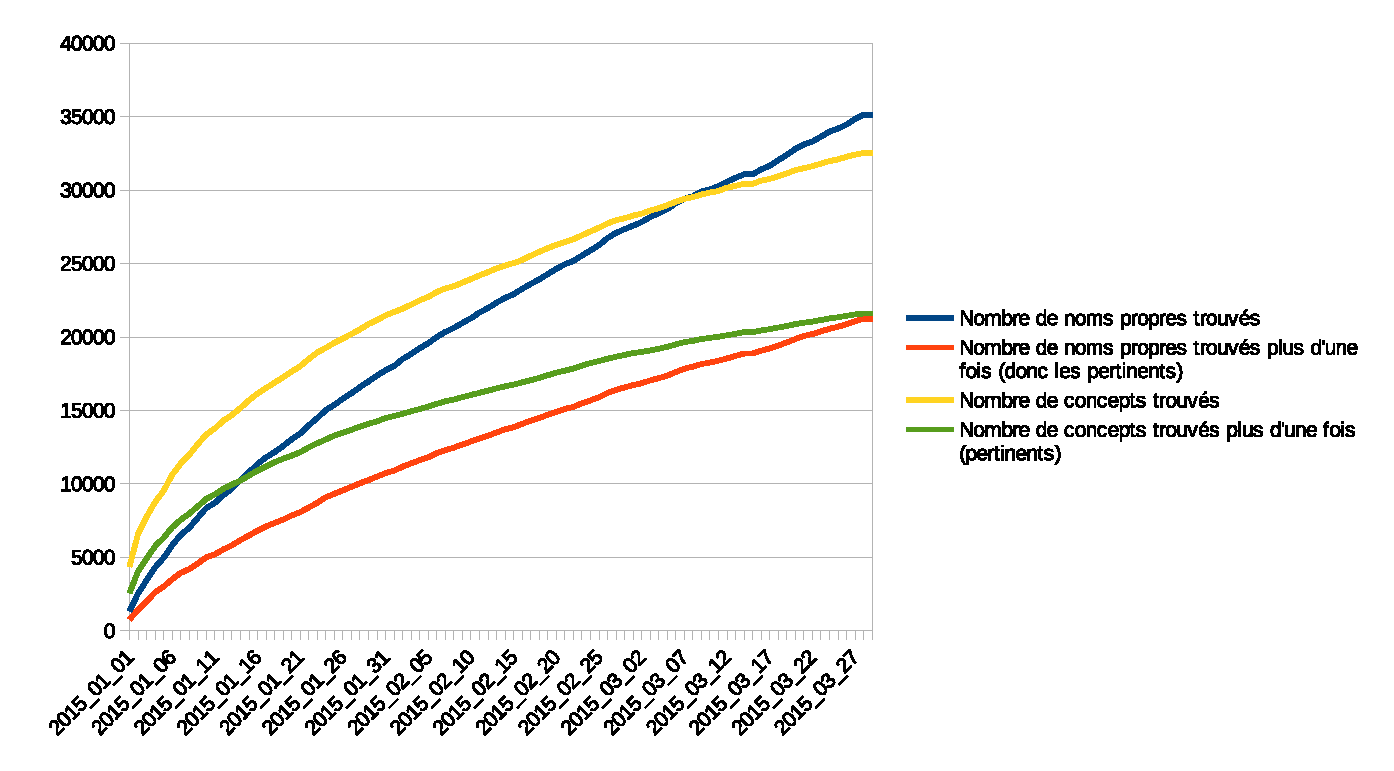
\includegraphics[width=16cm]{./conceptsnoms.eps}
 % conceptsnoms.eps: 0x0 pixel, 300dpi, 0.00x0.00 cm, bb=0 0 653 354
 \caption{\label{fig:conceptsnoms}Évolution en fonction du temps du nombre total de concepts et de noms propres tirés des articles}
\end{figure}



\subsection{WordNet}
%%reprise textuelle

WordNet est une base de données lexicale pour l'anglais, produite par l'université de Princeton.

Nous l'utilisons à travers son interface \pyt{nltk}, pour récupérer des informations sur les mots et les mettre sous forme normale.


\subsection{Conceptnet5}
%%reprise textuelle

Conceptnet (\href{http://conceptnet5.media.mit.edu/}{leur site}) est un projet libre de réseau sémantique représentant des connaissances usuelles, aussi bien de la vie de tous les jours que culturelles et scientifiques. Il fait partie du \ang{Commonsense Computing Initiative} qui relie différents laboratoires, dont le MIT Media Lab, et entreprises.

Il est important de noter que Conceptnet5\index{Concepnet5} est généré à partir de données brutes. Conceptnet5 est relié à DBPedia, une grande partie de ses connaissances provient de Wiktionary, une partie de WordNet.

Nous avons utilisé une partie de code source provenant de \href{https://github.com/commonsense/conceptnet5}{<github>}.


\subsubsection{Structure de Conceptnet5}
%%reprise textuelle

Conceptnet5\index{Conceptnet5} est un graphe sémantique\index{Graphe sémantique} contenant de l'ordre du million de nœuds et d'ar\^etes.

Les n\oe{}uds sont des mots et de courtes phrases, pas seulement en anglais (bien que pour notre projet, nous utilisions uniquement l'anglais). Les arêtes qui relient ces n\oe{}uds expriment une connaissance, elles contiennent chacune une relation particulière.

Une arête possède aussi une source (d'où provient l'information) et un poids en fonction de cette source, selon l'importance de l'arête.

Une relation concept-arête-concept exprime une assertion\index{Assertion}. Une même assertion peut être exprimée de différentes manières. Conceptnet5 contient 1.6 million d'assertions.

Une assertion peut elle-même être utilisée comme un n\oe{}ud ou comme une arête (on peut avoir des assertions d'assertions).

Les relations valables dans tout langage, pour Conceptnet5, sont par exemple~:
\begin{itemize}
 \item RelatedTo~;
 \item IsA~;
 \item PartOf~;
 \item MemberOf~;
 \item HasA~;
 \item TranslationOf~;
 \item DefinedAs\ldots{}
\end{itemize}

Il en existe beaucoup d'autres.

Comme Conceptnet est construit en partie à l'aide de WordNet, il existe une correspondance entre relations de l'un et de l'autre~:

La correspondance entre relations de WordNet et de Conceptnet est par exemple~:
\begin{itemize}
 \item attribute~: Attribute~;
 \item causes~: Causes~;
 \item classifiedByRegion~: HasContext~;
 \item hyponymOf~: IsA~;
 \item sameVerbGroupAs~: SimilarTo~;
 \item seeAlso~: RelatedTo.
\end{itemize}

Nous avons décidé après coup de conserver ces relations dans le réseau de concepts, et d'en utiliser un sous-ensemble. En effet, elles nous paraissent bien adaptées pour exprimer l'information que nous souhaitons voir contenue dans ce réseau.

\subsubsection{Détail de l'API (\ang{Application's Programmer Interface})}
%%reprise textuelle

Nous pouvons faire un certain nombre de requêtes à Conceptnet5. Il existe trois types différents de requêtes~:
\begin{itemize}
 \item \texttt{Lookup}~;
 \item \texttt{Association}~;
 \item \texttt{Search}~;
\end{itemize}
Association permet de calculer la proximité entre deux concepts, ou de récupérer une liste de concepts proches d'un concept donné.

\texttt{Search} permet de récupérer une liste d'arêtes (\ang{edges}) entre concepts, selon les paramètres spécifiés (le plus souvent, on impose le concept de départ \ang{start} ou d'arrivée \ang{end}).

\texttt{Lookup} permet d'analyser un concept (on aura par exemple accès à des listes d'arêtes dans lequel il intervient).


\subsubsection{Utilisation de Conceptnet5}

Nous utilisons en majorité \texttt{LookUp} et \texttt{Search}, les requêtes \texttt{Association} étant beaucoup plus lentes et ne pouvant être réalisées en temps tout à fait raisonnable sur des données mettant en jeu plusieurs milliers de requêtes.

Considérons un concept dont nous cherchons des voisins dans le réseau.
\begin{itemize}
 \item Une requête \verb|LookUp|\index{LookUp} nous donne déjà une idée desdits voisins (liens entrants ou sortants) ;
 \item Une recherche \verb|Search|\index{Search} précise pourra nous donner par exemple un certain nombre de voisins, par des liens sortants, que nous pourrons ajouter (en sélectionnant bien sûr les concepts jugés pertinents, selon quelques critères empiriques) ;
 \item Une requête \verb|Association|\index{Association} renvoie une liste de concepts similaires. On peut alors les relier au précédent avec un lien \verb|SimilarTo|.
\end{itemize}

\paragraph{Pertinence des concepts}
Conceptnet5 contient beaucoup d'information et les concepts sur lesquels il nous aiguille ne sont pas forcément pertinents. Il faut vérifier le poids des liens renvoyés, la similarité quand elle a lieu, ainsi que d'autres facteurs : nous ne pouvons pas garder les liens \verb|RelatedTo| car ils renvoient souvent à la traduction du mot dans une autre langue. Nous ne pouvons pas non plus garder les concepts formés d'une expression trop longue (atteignant parfois la taille d'une phrase entière), car celle-ci renvoie souvent à un événement ou un domaine très particulier, et sera de toute façon impossible à retrouver telle quelle dans un texte.


\subsection{Freebase}
%%reprise textuelle

Freebase\index{Freebase} est une immense base de données sémantiques qui contient beaucoup d'informations, sur des noms propres notamment. Le projet, repris par Google mais sous une licence qui laisse les données libres d'accès, de téléchargement et d'utilisation, a lui aussi une API, un peu plus complexe que celle de Conceptnet5. Freebase permet notamment de récupérer des informations sur une personne à partir de son nom, et à peu de frais, de vérifier que cette personne existe bel et bien.


\section{Réseau de concepts}\label{Section:RC}


\subsection{Cahier des charges}

Le réseau de concepts\index{Réseau de concepts} est la ``mémoire à long terme'' de notre programme. L'objectif est de disposer d'une représentation souple (sous forme de graphe sémantique) de données conceptuelles qui puissent ensuite être utilisées à mieux comprendre le texte lu.

Étant donné un concept (par exemple \verb|Wayne Rooney|), à quels autres concepts est-il relié et par quelles relations~? Il est essentiel, lorsque le texte ne contient pas suffisamment d'informations ou qu'elles ne sont pas exploitables (on n'a pas toujours ``vu'' à la lecture que Wayne Rooney était un nom propre ou un humain, par exemple), d'insérer ce type de données au cœur du processus de lecture. C'est pourquoi nous avons besoin du réseau de concepts.

D'autre part, nous pouvons exiger du résumé qu'il contienne une information explicite que le texte avait sous-entendu~; par exemple, que Wayne Rooney est un joueur de football. Le réseau devra donc contenir \verb|Wayne Rooney -> isA -> Soccer player|.

Ses prérogatives ont évolué au cours de notre projet. Au début, nous pensions faire reposer une plus grande partie de l'activité de résumé du texte sur lui (notamment par le processus d'activation et le repérage des nœuds activés), alors que celle-ci s'est dirigée ensuite sur le workspace\index{Workspace}.


\subsection{Structure du réseau de concepts}

\begin{definition}[Réseau de concepts]
Ce réseau est au carrefour entre les réseaux sémantiques\index{Graphe sémantique} et les réseaux de neurones. Les nœuds du réseau peuvent être vus comme représentant les concepts\index{Concept}.
\end{definition}

%%reprise textuelle
Le Réseau est constitué de n\oe{}uds. Chaque n\oe{}ud comporte~:
\begin{itemize}
  \item Une étiquette (mot) nommée concept\index{Concept}~;
 \item Une importance conceptuelle (ic) ou profondeur conceptuelle\index{Importance conceptuelle}~;
 \item Une activation (a)\index{Activation} initialement nulle~;
 \item Un certain nombre de liens à d'autres n\oe{}uds.
\end{itemize}

Chaque lien comporte~:
\begin{itemize}
 \item Une proximité conceptuelle\index{Proximité conceptuelle} (ou poids w)~;
 \item Une relation\index{Relation} qui le caractérise, prise sur le modèle de Conceptnet5\index{Conceptnet5}.
\end{itemize}

Ces différentes données numériques (proximité conceptuelle, activation, importance conceptuelle) sont normalisées entre $0$ et $100$.

\begin{figure}[h]
 \centering
 \includegraphics[width=14cm]{./rc_exemple.png}
 % rc_exemple.png: 812x612 pixel, 100dpi, 20.62x15.54 cm, bb=0 0 585 441
 \caption{\label{fig:rc_exemple}Exemple de réseau de concepts}
\end{figure}

\paragraph{}
Sur l'exemple de la figure~\ref{fig:rc_exemple}, nous revoyons les données qui nous intéressent. Les relations entre concepts sont exprimées de manière intuitive (\textit{Wayne Rooney IsA soccer player}, \textit{a soccer player is capableOf winning a match}). Nous ne représentons pas ici les poids, mais nous attendons d'eux qu'ils rendent compte du fait que si Wayne Rooney est effectivement un \textit{athlete}, il est plus pertinent de dire de lui qu'il est un \textit{soccer player}.


\subsection{Propagation d'activation}

\subsubsection{Principe}

Le réseau de concepts est dynamique. Il évolue au cours de la lecture du texte, notamment par un processus d'activation des n\oe{}uds. L'écoulement du temps est donc une donnée importante.

L'activation d'un mot (provoquée par exemple par sa lecture dans un texte) est propagée à tous les n\oe{}uds voisins. Elle permet intuitivement de penser à de nouvelles idées, de compléter l'information du texte si celle-ci est parcellaire.

Sur l'exemple de la figure~\ref{fig:rc_exemple}, l'activation du concept \verb|wayne_rooney| va provoquer dans un premier temps celle de \verb|soccer_player|, \verb|athlete|, mais aussi \verb|play_sport|, \verb|win_match|, etc.\\

La propagation d'activation doit tenir compte de plusieurs facteurs~: les poids des liens et l'importance conceptuelle des n\oe{}uds. Ainsi, un n\oe{}ud fortement relié à \verb|wayne_rooney| devra être activé plus rapidement et de façon plus importante.\\

Selon la manière dont nous voulons utiliser le réseau, il y a deux possibilités~:
\begin{itemize}
  \item Ou bien introduire un facteur de désactivation des n\oe{}uds au cours du temps, permettant éventuellement d'arriver à un état d'équilibre~;
 \item Ou bien rester en situation potentielle de déséquilibre (l'activation de chaque n\oe{}ud de la composante connexe ne cesse d'augmenter).
\end{itemize}

La notion de désactivation est assez satisfaisante intuitivement~; il existe en effet des concepts fortement activés mais peu importants, que l'on espère oublier assez rapidement. 

\subsubsection{Formalisation}
Formellement, nous utilisons les formules suivantes, inspirées de \cite{parmentier_specification_1998}.

\begin{itemize}
  \item Pour l'activation du n\oe{}ud $n$ à l'instant $t+1$~:
\begin{align}
 A_n^{t+1} = A_n^t + D^t + A^t
\end{align}
\item Pour la réactivation de ce n\oe{}ud~:
\begin{align}
 A^t = \sum_{(n' \rightarrow n \text{\ arcs entrants})} W_{(n'\rightarrow  n)} \times A_{n'}^t / 100
\end{align}
\item Pour la désactivation de ce n\oe{}ud~:
\begin{align}
 D^t = A^t \frac{100- IC_n}{100}
\end{align}
Où les facteurs $100$ sont dus à la normalisation. Si le concept a une très grande importance ($IC_n = 100$), il tend donc à ne pas être désactivé du tout. S'il a une importance très faible ($IC_n \rightarrow 0$), il a une tendance à se désactiver très rapidement.
\end{itemize}

\paragraph{}
Nous avons mis un temps plus important à extraire des importances conceptuelles véritablement utiles, et n'avons donc que peu utilisé la désactivation (qui repose sur l'importance conceptuelle). Ces importances conceptuelles ont été finalement calculées en nous inspirant de l'indice TF-IDF\index{TF-IDF}~; ce sera développé dans la partie~\ref{Section:TFIDF}.

\subsubsection{Facteur logarithmique}
Dans \cite{parmentier_specification_1998}, il était déjà question d'un facteur supplémentaire qui permette de tenir compte de la suractivation de n\oe{}uds fortement reliés. Effectivement, en l'absence de ce facteur supplémentaire, on remarque que des n\oe{}uds peu utiles mais fortement reliés (des mots et concepts courants comme \verb|person|, \verb|love|) vont rapidement être saturés, et dépasser les n\oe{}uds initiaux qui ont eux une grande importance.

Nous avons introduit ce facteur, et l'avons heuristiquement adapté. La formule d'activation d'un n\oe{}ud $n$ devient donc :
\begin{align}
 A_n^{t+1} = A_n^t + D^t + \frac{A^t}{divlog}
\end{align}
Où $divlog = \frac{\log(13 + \text{nombre d'arcs entrants})}{\log(13)}$.

Cela a donné des résultats très pertinents.

\subsubsection{Exemple}

Sur notre dernier et meilleur réseau de concepts, nous essayons par exemple d'activer simultanément deux concepts (\verb|wayne_rooney|, \verb|steven_gerrard|) et de propager cette activation :
\begin{itemize}
 \item Une fois :
 \begin{verbatim}
soccer_midfielder : 3
wayne_rooney : 60
athlete : 15
steven_gerrard : 60
person : 6
soccer_player : 15
 \end{verbatim}
 \item Deux fois, en oubliant les n\oe{}uds trop faiblement activés ($ < 5$) :
 \begin{verbatim}
  at_soccer_game : 6
wayne_rooney : 60
soccer_player : 12
break_record : 13
play_sport : 12
sport_event : 7
win_match : 6
head_ball : 9
steven_gerrard : 60
sprint : 9
jump_high : 13
athlete : 28
 \end{verbatim}
\item Quatre fois, en oubliant encore les n\oe{}uds trop faibles ($ < 10$) :
\begin{verbatim}
 sport_event : 13
player : 12
steven_gerrard : 60
athlete : 49
jump_high : 19
play_sport : 18
competition : 19
wayne_rooney : 60
sprint : 35
win : 21
break_record : 20
soccer_player : 10
\end{verbatim}
\end{itemize}
Nous pourrions aller plus loin, mais cela nous menacerait d'arriver à des n\oe{}uds fortement éloignés des deux sportifs initialement sélectionnés, et qui s'activeraient entre eux.


\subsection{Construction du réseau}
Comme cela a déjà été souligné plus haut, nous nous limitons au domaine du sport, domaine balayé par les articles qui constituent notre première source de données. 

La construction du réseau se déroule en différentes étapes, qui font intervenir quasiment toutes les sources de données de notre projet.


\paragraph{}
Certaines informations sur les éléments du réseau (poids des liens entre concepts notamment) sont relativement faciles à extraire des bases de données utilisées (Freebase, Conceptnet5 comportent déjà de telles informations, qu'il faut simplement renormaliser). En revanche, la seule manière probante d'obtenir une importance conceptuelle est de la calculer nous-mêmes.

Le réseau comporte à la fois des noms propres et des noms communs, des adjectifs, des verbes à l'infinitif~; des termes tout à fait courants (et qui ne sont pas inhérents au sport), comme des termes spécialisés.



\paragraph{Récupération de concepts et de noms}

Nous analysons un certain nombre d'articles, ici 17~000 issus de 7 flux rss différents sur 89 jours (quasiment l'intégralité des données de notre projet).


Nous avons écrit des \ang{tokenizers} adaptés aux contraintes techniques et erreurs d'écriture des données récupérées, qui viennent compléter ceux fournis par \pyt{nltk}.

Pour récupérer les noms propres, nous repérons à l'intérieur d'un article les mots marqués comme noms propres par le POS-tagger\index{Part-of-speech tagger} de \pyt{nltk}. Puis nous concaténons deux noms propres successifs. Enfin, nous retirons de la liste des noms propres ceux qui sont contenus à l'intérieur d'autres. Cette étape, largement sous-estimée au début, est cruciale puisqu'elle évite de considérer ``< nom + prénom >'' et ``<prénom>'' comme deux personnes différentes.

Nous comptons aussi la fréquence d'apparition de chaque nom et de chaque concept. 
On obtient 32~702 concepts et 35~488 noms. En réalité, un tiers d'entre eux sont des mots qui n'apparaissent qu'une seule fois, contenant par exemple des fautes d'orthographe, des néologismes ou résultant d'erreurs de notre part. On obtient par exemple~:
\begin{verbatim}
["aaron cresswell", 78]
["aaron creswell", 1]
\end{verbatim}
Ce qui suggère que dans l'un des articles trouvés, quelqu'un a commis une erreur sur le nom \verb|cresswell|. Nous éliminons donc les mots qui n'apparaissent qu'une fois. Cela nous laisse 27~070 concepts.

\paragraph{Traitement des noms avec Freebase}

Nous n'utilisons l'API Freebase que de fa\c{c}on assez simple. Chaque nom propre donne lieu à une requête. Si celle-ci aboutit, on analyse le résultat et si celui-ci comporte une donnée (exemple~: à l'envoi de \verb|"scott_jamieson"|, on récupère \verb|"soccer_midfielder"|), on ajoute un nouveau n\oe{}ud correspondant au réseau, et une arête \verb|IsA| dont le poids dépend du résultat de la requête.

L'importance conceptuelle d'un nom propre est prise par défaut comme importante.

\paragraph{Traitement des concepts avec Conceptnet5}

Chaque nouveau concept donne lieu à une requête de type \verb|Lookup|. Nous sélectionnons parmi les résultats les informations les plus pertinentes (en terme de poids, mais aussi en fonction des relations, que nous ne gardons pas toutes~: par exemple, \verb|RelatedTo| n'est pas une relation très pertinente, alors que \verb|IsA| est souvent pertinente).

L'importance conceptuelle allouée à un nouveau n\oe{}ud dépend pour beaucoup de sa fréquence d'apparition dans les articles.


\paragraph{Extension des nœuds du réseau}

Pour étendre les n\oe{}uds du réseau, nous sommes souvent amenés à chercher des liens partant d'un n\oe{}ud donné. Cela est effectué avec des recherches \verb|Search|. Nous pouvons aussi effectuer des requêtes \verb|Association| (bien que beaucoup plus lentes) afin d'induire de nouveaux liens avec des concepts similaires.



\paragraph{Suppression des nœuds inutiles}
%%reprise textuelle
Malgré les nombreux paramètres servant à filtrer, les requêtes n'ont pas donné des résultats toujours pertinents. Nous choisissons de retirer du réseau les nœuds faiblement reliés (un seul voisin). Ceux-ci seront de toute fa\c{c}on peu utiles lors de la propagation de l'activation.


\subsection{Exemple de réseau de concepts}

Nous avons eu l'occasion d'effectuer différents essais de construction du réseau de concepts et nous présenterons dans cette sous-section le dernier, qui a donné les résultats les plus intéressants.

\paragraph{Étape 1~: noms propres}

\begin{itemize}
 \item Les requêtes Freebase liées aux noms propres créent 10~405 n\oe{}uds dans le réseau, ainsi que 8~255 arêtes.
 \item On lance immédiatement des requêtes Search correspondant à tous les n\oe{}uds du réseau sur Conceptnet5, afin d'acquérir plus d'information~: on passe alors à 14~103 n\oe{}uds et 28~393 arêtes.
\end{itemize}

\paragraph{Étape 2~: concepts}

\begin{itemize}
 \item On lance une requête Lookup sur chaque concept trouvé dans les articles (27~070, les noms propres ont déjà été traités)~; on passe alors à 35~780 n\oe{}uds et 56~942 arêtes. Pour le moment, 18~762 n\oe{}uds sont certains d'être conservés (ce sont des résultats primaires de requêtes positives).
\end{itemize}


\paragraph{Étape 3~: Extension et élagage du réseau}

\begin{itemize}
 \item On étend alors l'ensemble des n\oe{}uds encore litigieux (17~018), en essayant de créer des liens vers des n\oe{}uds déjà existants, augmentant ainsi la connectivité du réseau. On passe à 76~497 arêtes.
 \item On regarde quels n\oe{}uds sont bien reliés à leur voisins, après cette opération. Au total, 28~583 n\oe{}uds semblent prometteurs.
 \item On supprime les autres n\oe{}uds. On obtient un réseau avec 28~583 n\oe{}uds et 69~307 arêtes.
\end{itemize}



\subsection{Choix de programmation du réseau de concepts}

Le réseau est enregistré sous forme de JSON Stream\index{JSON Stream}, un type de données repris à Conceptnet5, qui permet sans contrainte technique majeure de l'écrire sous forme facilement lisible par un utilisateur extérieur. Le nombre de nœuds étant resté raisonnable, nous n'avons pas eu à abandonner le package \pyt{networkx} qui nous permet de le représenter en mémoire sous forme de graphe.

\paragraph{}
Nous avons parallélisé les requêtes afin de les effectuer dans un temps raisonnable, même si l'opération de construction du réseau reste longue dans son ensemble (plus d'une heure) et que les quantités de données mises en jeu suggèrent qu'une utilisation différente, notamment de Conceptnet5 (téléchargement et recherche dans la base de données de façon locale), pourrait être faite.



\section{Méthodes statistiques avec TF-IDF}\label{Section:TFIDF}

La méthode statistique consiste à extraire des phrases par des techniques de la fouille de données textuelles. L'idée principale est de pondérer les phrases selon leur représentativité dans le texte et à afficher celles de poids le plus fort dans l'ordre de leur apparition dans le texte et dans la limite de la taille du résumé. Nous avons choisi ici l'indice TF-IDF pour mesurer ces poids.

\subsection{Algorithme statistique}

Pour donner à chaque phrase un poids, on cherche d'abord à mesurer l'importance de chaque mot. On a observé qu'il y a des mots qui se présentent presque dans tous les documents comme les articles, les auxiliaires etc. Donc il faut filtrer ces mots non-significatifs. Et d'autre part, les mots-clés d'un texte sont aussi des mots qui y sont fréquents et à qui doit donc être assigné un poids important.

On cherche donc ici un indice qui diminue selon le nombre d'apparitions dans tous les documents, et qui augmente selon le nombre d'apparitions dans le texte particulier. Et l'indice TF-IDF satisfait exactement ces critères.


\subsection{TF-IDF pour le résumé automatique}
Selon une lemme de Hans Peter Luhn, le poids d'un terme est propotionnel à son fréquence.

D'après la loi de Zipf, la fréquence d'occurrence $f(n)$ d'un mot est liée à son rang $n$ dans l'ordre des fréquences par une loi de la forme $f(n) = \frac{K}{n} $ où K est une constante.

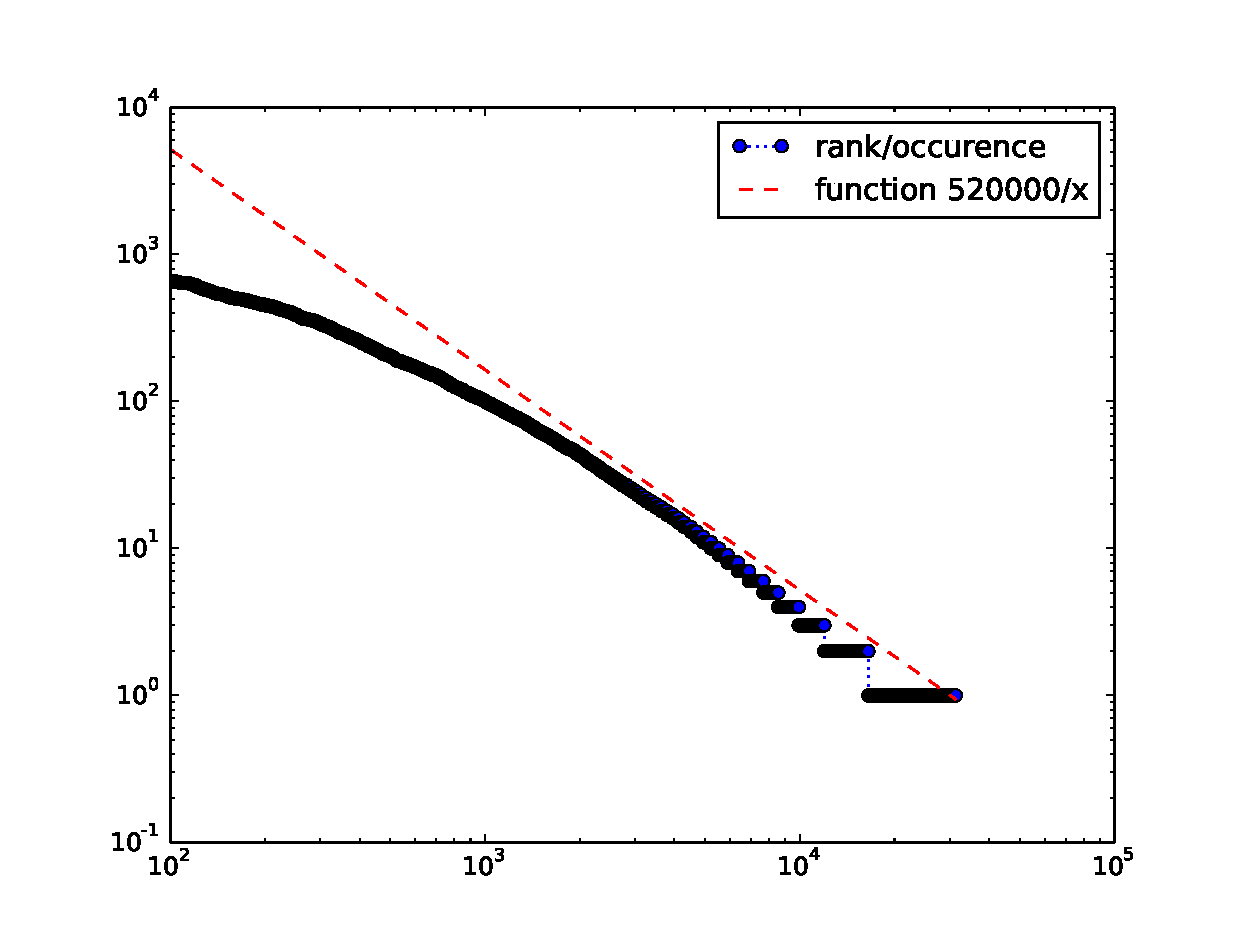
\includegraphics[scale=0.5]{loi_de_zipf.eps}

L'abscisse x est le rang d'un terme selon la fréquence et y est l'occurence de ce terme. Les mots plus fréquents sont 'the','of' et 'and'. On voit bien la courbe tend vers la fonction K/x.(ici on a choisi K = 5200000) C'est-à-dire que pour chercher les mots indiscriminant, il suffit de regarder l'inverse de la fréquence d'occurence.

\subsubsection{Définition formelle}

\begin{definition}[TF]
 La fréquence d'un terme (\textit{term frequency}, TF) que l'on mesure ici est juste le nombre d'occurrences de ce terme dans le document considéré.
\end{definition}

\begin{definition}[IDF]
 La fréquence inverse de document (\textit{inverse document frequency}, IDF) est une mesure de l'importance du terme dans l'ensemble du corpus. Elle vise à donner un poids plus important aux termes les moins fréquents, considérés comme plus discriminants.
\end{definition}

Ici, on prend la logarithme de cette fraction~:

\begin{align}
 idf_{i} =  log \frac{|D|}{|\{d_{j}: t_{i} \in d_{j}\}|}
\end{align}

Où : 
\begin{itemize}
 \item |D| est le nombre total de documents dans le corpus ;
 \item $|\{d_{j} : t_{i} \in d_{j}\}|$ est le nombre de documents où le terme  $t_{i}$  apparaît (c'est-à-dire  $n_{i,j} \neq 0$)
\end{itemize}

Plus un mot apparaît, plus son indice IDF tend vers zéro. Des mots qui sont présents dans tous les documents vont notamment être filtrés car ils ont un indice nul.

\begin{definition}[TF-IDF]
Le poids du mot s'obtient en multipliant les deux mesures TF et IDF.
\end{definition}

\begin{align}
 tfidf_{i,j} = tf_{i,j} \cdot  idf_{i}
\end{align}

\begin{definition}[Poids d'une phrase]
Après avoir calculé les indices TF-IDF de chaque mot dans une phrase, on les somme et divise cette somme par le nombre de mots dans cette phrase : c'est le poids de cette phrase (on oubliera bien sûr les phrases trop courtes, moins de deux concepts, pour lesquelles le poids peut être défini comme nul).
\end{definition}

\subsubsection{Illustration}
Voyez le tableau de valeur TF-IDF de 4 termes dans 3 documents sur un corpus de 1000 documents.
\begin{center}
	\begin{tabular}{|c|c|c|c|c|}
	 \hline
	 	Terme & tf(document 1) & tf(document 2) & tf(document 3) & idf \\
	 \hline
	 	he & 90 & 61 & 63 & 0.006 \\
	 \hline
	 	on & 43 & 34 & 51 & 0.008 \\
	 \hline
	 	discussion & 11 & 0 & 0 & 6.39 \\
	 \hline
	 	traveller & 0 & 13 & 0 & 6.39 \\
	 \hline
	\end{tabular}
\end{center}

Et les TF-IDF de ces 4 termes se calculent comme ci-dessous:

\begin{center}
	\begin{tabular}{|c|c|c|c|}
	 \hline
	 	Terme & TF-IDF(document 1) & TF-IDF(document 2) & TF-IDF(document 3) \\
	 \hline
	 	he & 0.540 & 0.366 & 0.378 \\
	 \hline
	 	on & 0.344 & 0.272 & 0.408 \\
	 \hline
	 	discussion & 70.29 & 0 & 0 \\
	 \hline
	 	traveller & 0 & 83.07 & 0 \\
	 \hline
	\end{tabular}
\end{center}

On voit ici l'influence de la fréquence inverse sur le TF-IDF: dans le document 1, même si le terme 'he' est plus fréquent que celui de 'dicussion', son indice TF-IDF est petit, car il apparaît dans la plupart des documents et a un indice IDF petit. Pour le document 1, 'discussion' est plus discriminant que 'he'.

\paragraph{}
Après avoir obtenu les valeurs TF-IDF de chaque terme, on peut calculer les poids de chaque phrase. Notre résumé est construit en additionnant la première phrase du texte (souvent le titre, qui, riche en information, a souvent le meilleur poids) avec quelques autres ayant un poids maximal, prises dans leur ordre d'apparition dans le texte.

On peut ainsi facilement agir sur la longueur du résumé par rapport à celle du texte (ne sélectionner qu'une phrase sur trois, ou sur quatre).

\subsection{Tests et qualité des résumés obtenus}

La qualité des résumés obtenus par la méthode TF-IDF est peu optimale. En effet, avec un regroupement simple de phrases, on perd beaucoup d'information contextuelle. Par exemple, on peut avoir souvent une phrase commençant par un mystérieux \textit{he} (il) ou \textit{she} (elle). Et cette phrase sans contexte est souvent peu compréhensible. (C'est aussi pour cela que nous choisissons d'inclure dans le résumé la première phrase, car elle contient \textit{a minima} les noms des personnes dont l'article parle).

Deux exemples sont disponibles en annexe \ref{Annexe:resumes}.

%En revanche, pour la recherche des mots-clés, la méthode TF-IDF est assez efficace. Nous avons remarqués qu'à partir de ces mots-clés, à l'aide d'une méthode synthétique, nous pouvons construire des phrases plus claires et éventuellement faire un résumé du texte. ??

\subsection{TF-IDF pour l'importance conceptuelle}

Dans un premier temps, l'importance conceptuelle\index{Importance conceptuelle} n'était définie que de manière floue et n'était pas dérivée d'informations quantitatives autres que des fréquences d'apparition de concepts (des concepts apparaissant plus souvent étant favorisés).

Nous avons donc adapté l'indice TF-IDF pour calculer une importance conceptuelle. Cela a même pu être adapté aux noms propres.

L'idée est que les termes ayant une importance conceptuelle forte sont ceux qui~:
\begin{itemize}
 \item Ont une fréquence (TF) élevée ;
 \item Et une occurence faible, c'est-à-dire qu'on ne les trouve pas partout.
\end{itemize}


La différence avec le calcul précédent de TF-IDF est que le TF était calculé de manière locale à un document, alors qu'ici, il est calculé de manière globale, étant donné que nous ne nous positionnons pas sur un document en particulier.

\paragraph{}
Ce calcul est effectué d'une part sur les noms propres, d'autre part sur les concepts (nous n'avons pas cessé depuis le début de séparer les uns et les autres). L'intérêt reste toujours le même : pour les noms propres, cela va rendre compte de l'importance qu'a chaque personne. De manière générale, les TF globaux des concepts sont beaucoup plus importants que ceux des noms propres, et les IDF sont beaucoup plus faibles : lorsqu'il apparaît, un nom propre apparaît moins fréquemment et dans un moins grand nombre de documents.

Le résultat est un TF-IDF très important pour certains concepts, même par rapport aux meilleurs noms, nous faisant conclure qu'une renormalisation différente (pour transformer en un indice entre 0 et 100) pour les deux catégories sera nécessaire.

\paragraph{}
Une partie représentative des résultats est reproduite en annexe \ref{Annexe:TFIDF}.

On remarque notamment, dans le cas des noms propres, que les faux noms propres (erreurs de POS-tagging) se sont retrouvés en bas du tableau. En effet, même lorsqu'ils apparaissent plusieurs fois, ce sera dans plusieurs textes distincts, alors qu'un véritable nom propre à même fréquence aura tendance à apparaître plusieurs fois dans le même document.


\section{Traitement préalable des données}

Pour assurer une certaine cohérence entre les données présentes dans le réseau de concepts et celles présentes dans le workspace, il est bien sûr nécessaire de faire le même travail de normalisation qui a eu lieu lors de la construction du premier. Cependant, le workspace étant destiné à contenir des informations beaucoup plus précises et ciblées sur un texte que le réseau, il est nécessaire de faire un travail préalable sur les données du texte avant des les introduire dans le workspace. Ces étapes sont décrites ci-dessous et se regroupent en deux parties : une analyse syntaxique, d'une part, permettant d'établir les liens entre les différents éléments du texte ; et d'autre part un travail sur la reconnaissance des pronoms permettant de distinguer les différentes entités présentes dans le texte.

\subsection{Analyse syntaxique}\index{Analyse syntaxique}

Cette partie ne constituant pas le c\oe{}ur de notre PSC, nous avons décidé d'utiliser un outil déjà codé. L'entreprise Systran, au sein de laquelle notre tuteur travaille, a accepté de traiter nos données et nous a renvoyé un graphe sémantique contenant une analyse syntaxique complète des articles du corpus..

\subsubsection{Description algorithmique d'une grammaire}\index{Grammaire}
Une grammaire peut être décrite informatiquement de manière très simple. En effet, on peut la voir comme~:
\begin{itemize}
	\item Un ensemble de classes terminales (verbe, nom par exemple) associées à une liste de mots ou éventuellement d'expressions
	\item Un ensemble de règles, souvent sous la forme d'une reconnaissance de motifs, permettant de découper une phrase en plusieurs éléments (et finalement en unités syntaxiques élémentaires).
\end{itemize}

Il y a par conséquent deux manières pour une grammaire d'être incomplète~: soit elle ne connaît pas assez de vocabulaire (manque d'éléments dans les cas terminaux), soit elle ne connaît pas assez de règles. La première faille est assez facile à combler par des requêtes vers WordNet\index{WordNet} (et par ailleurs un outil automatique est inclus dans \pyt{nltk}\index{Natural Language ToolKit})~; il est en revanche assez indispensable d'avoir une grammaire complète en termes de règles car il est beaucoup plus difficile d'inventer des manières de découper une phrase.

Il est également à noter que les grammaires modernes s'appuient sur un entraînement statistique et traite les données de manière stochastique.

\subsubsection{\'Etat du texte en fin d'analyse}
Les données traitées par Systran nous sont revenues sous la forme d'un graphe sémantique. Chaque nœud, ou mot, de la phrase était de plus enrichi d'une liste de tags permettant d'établir de quel genre de mot il s'agit (humain, véhicule, lieu si c'est un nom; verbe d'action, verbe descriptif si c'est un verbe; etc.) Notons également que chaque nœud contient une liste (éventuellement vide) de fils avec lesquels il forme une entité syntaxique cohérente telle qu'un groupe nominal. Cela nous a été très utile lorsqu'il s'est agit de faire la différence entre les entités et leurs attributs lors de leur incorporation dans le workspace.

Par commodité, nous avons d'abord transformé ces données au format JSON avant des les inclure dans le workspace.

\subsection{Résolution de pronoms}

Le but de la résolution de pronoms\index{Résolution de pronoms} est, étant donné une phrase qui peut être par exemple~:

\begin{verbatim}
 Sepp_+_Blatter is the favourite to win a Fifa race he vowed he would not stand for.
\end{verbatim}
de rapporter chaque pronom à un groupe nominal. Ici, les deux pronoms que l'on repère (``he'') se rapportent évidemment à \verb|Sepp_+_Blatter|.

Nous disposons pour nous aider des données fournies par l'analyseur syntaxique de Systran. En voici une liste non exhaustive~:
\begin{itemize}
 \item POS\index{Part-of-speech}
 \item Type grammatical de chaque mot~: nom propre, acronyme, verbe, auxiliaire, préposition\ldots{}
 \item Différents liens entre les mots~: adjectif relié à un nom, article\ldots{}
\end{itemize}


\subsubsection{Étape 1}
On commence par trouver l'ensemble des groupes nominaux. Nous avons deux choix~:
\begin{itemize}
 \item Ou bien les trouver tous~;
 \item Ou bien se limiter d'emblée à ceux qui ont leurs chances.
\end{itemize}

Nous prenons d'abord le deuxième choix~: l'analyseur de Systran nous indique en particulier, étant donné un mot, s'il est objet ou sujet d'un verbe. Nous considérons donc, dans un premier temps, que les noms concernés sont les noms principaux et que tous les groupes nominaux qui nous intéressent se construisent autour d'eux.

Après expérience, nous avons étendu le ``droit'' de créer un groupe nominal à de simples compléments d'objet, constatant qu'ils apparaissaient eux aussi.


\subsubsection{Étape 2}
On considère maintenant l'ensemble des pronoms.

Pour un pronom situé à une position donnée, les groupes nominaux\index{Groupe nominal} potentiels font l'objet d'un classement, relatif à un score, que nous calculons de la manière suivante~:

\begin{itemize}
 \item Un candidat a le droit d'être situé dans une phrase précédente (sous une limite fixée à 2 ou 3). Plus il est éloigné du pronom, plus son score diminue. S'il est après le pronom, son score diminue drastiquement (voire $-\infty$).
 \item Le candidat doit vérifier certaines correspondances avec le pronom~: en particulier, il doit avoir le même genre et le même nombre. Si c'est vérifié, le score augmente. Sinon, le score diminue. Cette information n'est pas tout le temps disponible. En revanche, on sait parfois si le groupe nominal concerné (son nom principal) est un humain ou non.
 \item On a parfois (notamment avec le pronom ``that'') de manière directe l'information de l'antécédent. L'antécédent désigné doit alors gagner un score énorme (voire $+\infty$, mais l'analyseur de Systran n'est pas infaillible).
 \item Un groupe nominal qui apparaît au début d'une phrase doit, quels que soient les pronoms, avoir un meilleur score. Les noms propres apparaissent souvent au début de la phrase pour être ensuite rappelés par des pronoms, c'est d'ailleurs le cas dans l'exemple ci-dessus.
 \item Un groupe nominal répété gagne également en score.
 \item Un groupe nominal précédé d'une préposition perd en score.
 \item Un groupe nominal sujet gagne en score, et un groupe objet perd en score. 
 \item Un groupe nominal comportant un article indéfini perd en score.
 \item Un groupe nominal comportant un nom propre gagne en score.
\end{itemize}

Ces différentes exigences satisfont à un impératif de simplicité. On cherche ensuite à balancer le mieux possible les augmentations/diminutions de score afin de maximiser la pertinence des résultats.

Nous nous inspirons pour cette méthode de \cite{Mitkov:1998:RPR:980691.980712}, pour sa simplicité et son adaptabilité quant aux données dont nous disposons.


%%%%%%%%%%%%%%%%%%%%%%%%%%%%%%%%%%%%%%%%%%%%%%%%%%%%%%%%

%%%%%%%%%%%%%%%%%%%%%%%%%%%%%%%%%%%%%%%%%%%%%%%%%%%%%%%ù

%%%%%%%%%%%%%%%%%%%%%%%%%%%%%%%%%%%%%%%%%%%%%%%%%%%%%%%ù

\section{Traitement du réseau}

Le réseau de concepts représente, comme nous l'avons déjà dit, la connaissance \textit{a priori} de notre programme sur le domaine étudié. Pour étudier un texte particulier, il s'agit maintenant de faire agir ce texte sur nos connaissances et d'interpréter l'effet que cette lecture a.

Deux méthodes ont été envisagées~: la première étudiait, essentiellement, la différence entre l'état du réseau de concepts avant et après la lecture et devait en déduire les faits importants. La seconde, qui a finalement été retenue, s'appuie sur une activation des concepts dans le réseau, puis une instanciation des concepts fortement activés dans un espace de travail appelé \textit{workspace}\index{Workspace}. Ces concepts instanciés sont par la suite capable d'effectuer des tâches plus complexes relatives à la compréhension du texte.

Quelle que soit la méthode employée, une analyse syntaxique\index{Analyse syntaxique} préalable du texte est nécessaire pour rendre compte de sa compréhension et utiliser au mieux notre réseau de connaissances.

\subsection{Workspace}\index{Workspace}
Le Workspace est une zone où on va stocker des structures formées à partir de concepts et travailler dessus. Par opposition au réseau de concepts, qui représente une connaissance relativement figée du monde, ces structures visent à représenter la compréhension que l'on a pu acquérir du texte.
Par exemple, un type de structure rencontré dans le Workspace serait un graphe décrivant l'évolution de l'état d'un objet au fur et à mesure du temps, d'après ce qu'on a pu extraire du texte.

\subsubsection{Structure du Workspace}
Comme on l'a dit il s'agit essentiellement d'une structure de graphe orienté.

Les nœuds représentent des concepts présents dans le texte à résumer ou bien des concepts qui lui sont liés. On différencie ces concepts en deux sous-classes, selon qu'il s'agit d'entités ou d'attributs.

\begin{definition}[Entité]
On parle d'entité pour désigner une chose ou une personne formant une unité, réelle ou non, capable d'agir ou de subir des actions dans le cadre du texte. Un fantôme ou une voiture sont des entités ; deux voitures forment deux entités distinctes ; et la joie (par exemple) n'est pas considérée comme une entité.
\end{definition}
\begin{definition}[Attribut]
Un attribut est un concept altérant ou complétant le sens d'un autre. Par exemple, "Angleterre" dans "l'équipe d'Angleterre" est un attribut de "l'équipe". L'attribut n'ayant pas de sens à lui seul, on parlera toujours de l'attribut de telle entité.
\end{definition}

On voit déjà sur ces exemples simples que la distinction entre entité et attribut n'est pas triviale. En effet, dans un contexte différent, l'Angleterre pourrait être considérée comme une entité. Elle est pourtant essentielle à la compréhension du texte, et donc à son résumé, dans la mesure où ce seront les entités qui seront le sujet du texte.

De plus, les structures du Workspace doivent être capables de rendre compte des actions effectuées ou subies par les entités. Pour cela, il nous a semblé plus facile d'étudier l'effet qu'ont ces actions sur l'état des entités : on parle alors d'évènement.

\begin{definition}[État]
L'état d'une entité désigne l'ensemble de ses attributs à un moment donné.
\end{definition}
\begin{definition}[Évènement]
Un évènement est une arête dans le graphe présent dans le workspace, reliant une entité ou un attribut à un autre. Si l'origine est une entité, il représentera le plus souvent une action ; si l'origine et la destination sont des attributs il représentera plutôt un changement dans l'état de l'entité à laquelle ils sont reliés.
\end{definition}

\subsubsection{Implémentation}

Pour l'implémentation, on utilise une seule classe python contenant pour seul champ une liste de concepts. Ces concepts sont des instantiations d'une classe abstraite, dont héritent trois classes \pyt{Entity}, \pyt{Attribute} et \pyt{Event}.

%% Copier (un bout de) le code ?

\subsubsection{Utilisation}

Le fait d'ajouter des liens syntaxiques et logiques (par les évènements) entre les concepts intervenant dans le texte nous permet d'accéder de manière assez directe à leur importance relative dans le texte. En effet, du point de vue syntaxique, un concept fortement connecté sera présent dans une grande partie du texte et pourra donc être considéré comme le sujet, au moins du point de vue de l'auteur du texte, de ce dernier. Si, qui plus est, une entité ou ses attributs est l'origine ou la destination de nombreux évènements, il constituera un point central du texte au niveau du contenu.

Ainsi l'importance d'un concept tant du point de vue de la forme que du fond nous semble directement relié à la connectivité des entités dans le graphe. L'algorithme de résumé procède donc comme suit :
%% Bon je suis un peu flou sur les détails.

\begin{enumerate}
	\item On parcourt le graphe sémantique représentant le texte et, pour chaque mot, selon qu'il est entité ou attribut, le plonge à l'endroit idoine du workspace.
	\item Les concepts proches des concepts très connectés sont ensuite plongés dans le workspace et reliés au reste.
	\item On réduit ensuite le graphe en élaguant les nœuds moins connectés.
	\item Les quelques nœuds restants sont présentés au lecteur.
\end{enumerate}

%% À vérifier
Même si le résultat final n'est pas une phrase intelligible, les informations présentes dans la sortie doivent être suffisantes pour permettre au lecteur de se faire une idée de l'évènement principal dont traite l'article.


\section{Bilan et améliorations envisageables}


%% J'espère pouvoir corriger ce paragraphe dans les prochains jours
Le projet n'a que peu de retard sur ce qui a été annoncé. Le workspace a été presque entièrement implémenté et nous sommes capables d'y introduire un texte en structures cohérentes. Nous avons cependant manqué de temps pour implémenter les parties les plus subtiles de nos algorithmes (étoffement des liens dans le workspace).

\subsection{Considérations techniques}

Le code de notre projet, de grande taille, est entièrement documenté.

\subsection{Bilan des actions menées}

Dans son état actuel, le projet constitue une excellente préparation à la mise en place des méthodes que nous avons décrites. Nous avons en effet améliorés quelques outils de traitement de données textuelles brutes (en ce qui concerne le traitement des noms propres notamment). Nous avons également pu mettre en place les structures indispensables à nos algorithme et créé les fonctions faisant l'interface avec les structures de données déjà existantes.

Nous avons, d'autre part, pu implémenter un algorithme raisonnable de résumé automatique s'appuyant sur TF-IDF. % Complement needed.



\vspace{1\baselineskip}

%\subsection{Améliorations}

%\subsubsection{Apprentissage du réseau de concepts}
%Le réseau de concept représente un \textit{a priori} sur le monde de notre programme. Il est donc normal que cette structure évolue au fur et à mesure des textes lus.

%Les fonctions de construction du réseau peuvent sans mal être appelées après la génération du résumé pour y apporter des modifications pérennes, que ce soit sur les données brutes ou, mieux encore, sur les structures encores présentes dans le workspace qui contiennent explicitement des relations entre les différents concepts présents.


%\subsubsection{\'Evaluation des résumés}
%Le faible nombre de résumés que nous prévoyons de produire nous permettra d'utiliser la méthode la plus simple parmi celles qui étaient mentionnées dans la proposition détaillée~: la comparaison à un résumé déclaré bon car produit par un humain.

%L'idée est la suivante~: l'un de nous résumera un texte, nous emploierons notre programme pour résumer le même texte, et enfin nous utiliserons un simple algorithme statistique (basé sur TF-IDF) pour résumer ce même texte. Nous comparerons ensuite ces résumés du point de vue de l'information qu'ils contiennent~: sont-ils des images assez fidèles du document original~?

%Compte-tenu de la simplicité de l'algorithme statistique, nous espérons que le résumé produit par notre programme se situera quelque part entre le résumé statistique et le résumé humain.



 

\section{Références bibliographiques}

\begin{quotation}
 This work includes data from ConceptNet 5, which was compiled by the Commonsense Computing Initiative. ConceptNet 5 is freely available under the Creative Commons Attribution-ShareAlike license (CC BY SA 3.0) from http://conceptnet5.media.mit.edu. The included data was created by contributors to Commonsense Computing projects, contributors to Wikimedia projects, Games with a Purpose, Princeton University's WordNet, DBPedia, OpenCyc, and Umbel.
\end{quotation}

\nocite{*}
\printbibliography{}

\newpage
\appendix

\section{Indices TF-IDF pour certains concepts et noms propres}

Les indices reproduits ci-dessous ne sont pas normalisés.

\begin{figure}[!h]
\begin{center}
 \begin{tabular}{|c|c|}
 \hline
  \textbf{Terme} & \textbf{TF-IDF} \\
  \hline
  goal & 18036.355588902752 \\
  club & 16707.84340604437 \\
  win & 16416.987149003868 \\
  player & 15395.13561971935 \\
  do & 14983.099117885753 \\
  get & 14831.125247005852 \\
  game & 14772.460116022885 \\
  team & 14736.039158065283 \\
  season & 14410.376362720359 \\
  score & 14347.834720380053 \\
  fan & 14345.794404055676 \\
  ball & 14183.767993101164 \\
  say & 14041.53077169254 \\
  play & 13932.858353857095 \\
  go & 13866.246326872366 \\
  share & 13220.473403693579 \\
  year & 13048.180880727492 \\
  football & 12974.031162373381 \\
  time & 12476.391302456212   \\
  right & 12370.950387951321     \\
  think & 12340.221480751856   \\
  first & 12325.427075870062   \\
  watch & 12318.296129723469   \\
  last & 12292.45714341061   \\
  match & 12258.013990918109   \\
  side & 12245.076493840706   \\
  leave & 12133.864922485838   \\
 $\cdots$ & $\cdots$ \\
    kangaroo  & 9.025515684964109  \\
  q  & 8.620050576855945  \\
  wristband  & 8.620050576855945  \\
  fifteenth  & 8.620050576855945  \\
  refinance  & 8.620050576855945  \\
  wishy-washy  & 8.620050576855945  \\
  inheritance  & 8.620050576855945  \\
  annex  & 8.332368504404164  \\
  featherweight  & 8.332368504404164 \\
  \hline
 \end{tabular}
\label{fig:TFIDFConcepts}
\caption{Extrait de la base de données de TF-IDF pour des concepts}
\end{center}
\end{figure}


\begin{figure}[!h]
\begin{center}
 \begin{tabular}{|c|c|}
 \hline
  \textbf{Nom} & \textbf{TF-IDF} \\
  \hline
  chelsea  & 15435.05496583199 \\
  premier league  & 14572.723366675536 \\
  liverpool  & 14412.6737426319 \\
  foul  & 10777.070534251237 \\
  steven gerrard  & 9402.731890649875 \\
  louis van gaal  & 9163.915519209326 \\
  cup  & 9132.154367268871 \\
  attempt  & 8675.8177744147 \\
  barcelona  & 8578.435422472256 \\
  england  & 8278.73616736681 \\
  lionel messi  & 7657.736882963432 \\
  harry kane  & 7460.74448794179 \\
  cristiano ronaldo  & 7375.310093934143 \\
  tottenham  & 7119.794079790657 \\
  burnley  & 5942.596160930355 \\
  league  & 5847.736458560602 \\
  diego costa  & 5674.059267902648 \\
  wayne rooney  & 5382.705157188505 \\
  radamel falcao  & 5141.135765623698 \\
  gareth bale  & 4761.904077325407 \\
 $\cdots$ & $\cdots$ \\
  whet  & 9.718662865524054 \\
  embrace  & 9.718662865524054 \\
  oar  & 9.718662865524054 \\
  autograph  & 9.718662865524054 \\
  faith  & 9.718662865524054 \\
  attitude  & 9.718662865524054 \\
  place  & 9.025515684964109 \\
  blueprint  & 9.025515684964109 \\
  ergo  & 9.025515684964109 \\
  subscribe  & 9.025515684964109 \\
  bold  & 9.025515684964109 \\
  hear  & 9.025515684964109 \\
  thing  & 9.025515684964109 \\
  ohio  & 9.025515684964109 \\
  lanky  & 9.025515684964109 \\
  mustapha carayol  & 9.025515684964109 \\
  innocent  & 9.025515684964109 \\
  count  & 9.025515684964109 \\
  detroit  & 9.025515684964109 \\
  our  & 8.620050576855945 \\
  not  & 8.620050576855945 \\
  fenway park  & 7.926903396296 \\
  \hline
 \end{tabular}
\label{fig:TFIDFNoms}
\caption{Extrait de la base de données de TF-IDF pour des noms propres}
\end{center}
\end{figure}

\section{Exemples de résumés avec une méthode statistique}

\subsection{Texte 1}

Tiré du site de \href{http://www.theguardian.com/football/2015/mar/29/georgia-germany-euro-2016-match-report}{\textit{The Guardian}}, le 29 mars 2015.

(Notons une erreur survenue dans la récupération de l'article : la légende de l'image a été prise comme faisant partie du texte.)

\begin{quotation}
Germany's Marco Reus,  right,  celebrates his goal against Georgia.\\
Photograph.\\
David Mdzinarishvili/ REUTERS.\\
The World Cup winners Germany eased past the hosts Georgia 2-0 in their Euro 2016 qualifier on Sunday with first-half goals from Marco Reus and Thomas Müller enough to get their Group D campaign back on track.\\
Reus put the visitors ahead after 39 minutes and Müller doubled their lead before the break as the Germans,  who had an erratic start to the qualifiers last year when they lost in Poland,  were never threatened by their weaker opponents.\\
The win lifted Germany,  who did not need to hit top form,  to 10 points from five games to equal Poland,  who take on Ireland later on Sunday,  and Scotland.\\
Georgia have had a tough start in Group D,  recording four defeats and a win in Gibraltar to stay on three points.\\
It did not take long for Germany,  with several World Cup winners back in the squad including captain Bastian Schweinsteiger,  to threaten and Reus’ powerful drive was palmed on to the crossbar by the keeper Giorgi Loria after five minutes.\\
With the coach Joachim Löw reverting to a four-man defence from a three-player experiment against Australia in a friendly on Wednesday,  Germany pressured their opponents’ box for most of the first half.\\
Müller fired at goal directly from a corner only to see the ball fly just wide of the post and Mesut Özil missed another big chance as the visitors had the hosts firmly on the backfoot.\\
Reus did better in the 39th when Mario Götze charged into the box and was lucky to scramble the ball to the winger,  who drilled home for his second goal this week after also scoring in their 2-2 friendly draw against Australia.\\
Müller then added another on the stroke of halftime to firmly put Germany in the driving seat.\\
The new Georgia coach Kakhaber Tskhadadze added a forward after the break but it was Reus who came close again,  rattling the bar for a second time on the hour with another powerful shot.\\

\end{quotation}

\subsection{Phrases du texte 1 par poids décroissants}

\begin{quotation}
 ( The win lifted Germany,  who did not need to hit top form,  to 10 points from five games to equal Poland,  who take on Ireland later on Sunday,  and Scotland. , 8242.26772072029)\\
( Reus did better in the 39th when Mario Götze charged into the box and was lucky to scramble the ball to the winger,  who drilled home for his second goal this week after also scoring in their 2-2 friendly draw against Australia. , 7825.67291347488)\\
( Georgia have had a tough start in Group D,  recording four defeats and a win in Gibraltar to stay on three points. , 7096.286506924158)\\
("Germany s Marco Reus,  right,  celebrates his goal against Georgia.", 7081.905602739567)\\
( Müller fired at goal directly from a corner only to see the ball fly just wide of the post and Mesut Özil missed another big chance as the visitors had the hosts firmly on the backfoot. , 6985.560661733021)\\
( Photograph. , 6066.563168646177)\\
( The new Georgia coach Kakhaber Tskhadadze added a forward after the break but it was Reus who came close again,  rattling the bar for a second time on the hour with another powerful shot. , 5585.593141599327)\\
( Reus put the visitors ahead after 39 minutes and Müller doubled their lead before the break as the Germans,  who had an erratic start to the qualifiers last year when they lost in Poland,  were never threatened by their weaker opponents. , 5286.39283077408)\\
( It did not take long for Germany,  with several World Cup winners back in the squad including captain Bastian Schweinsteiger,  to threaten and Reus’ powerful drive was palmed on to the crossbar by the keeper Giorgi Loria after five minutes. , 3877.015426088277)\\
( The World Cup winners Germany eased past the hosts Georgia 2-0 in their Euro 2016 qualifier on Sunday with first-half goals from Marco Reus and Thomas Müller enough to get their Group D campaign back on track. , 3873.7065644920067)\\
( With the coach Joachim Löw reverting to a four-man defence from a three-player experiment against Australia in a friendly on Wednesday,  Germany pressured their opponents’ box for most of the first half. , 3791.76236469219)\\
( Müller then added another on the stroke of halftime to firmly put Germany in the driving seat. , 3071.837346062652)\\
\end{quotation}


\subsection{Texte 2 (extrait)}

Tiré également du \href{http://www.theguardian.com/football/2015/mar/29/northern-ireland-finland-euro-2016-qualifier-match-report}{site de \textit{The Guardian}}.

\begin{quotation}
 Kyle Lafferty,  right,  celebrates with his Northern Ireland team-mates after scoring the first goal against Finland . \\
Photograph . \\
Andrew Paton/ EPA . \\
Kyle Lafferty exhibited precisely why he is at the vanguard of this seismic Northern Ireland renaissance,  after helping to sink Finland’s hopes of qualification for Euro 2016
The rangy striker may be lounging at the on-loan Turkish outpost of Caykur Rizespor,  but the Norwich City man came alive when needed at Windsor Park . \\

[...]\\

But it was sufficient to settle nerves amongst the Green and White Army . \\
Finland,  reeling,  must have felt their pockets had been picked . \\
O’Neill sent out a more focused,  organized outfit in the second half,  taking control of most situations . \\
A sense of calm restored,  with Finland having lost their earlier verve . \\
The visitors did recover slightly,  helping themselves to an injury time consolation with Sadik lashing home to shred home nerves . \\
Nonetheless it will be a relieved O’Neill looking forward to matters with massive optimism . \\
\end{quotation}

\subsection{Résumé du texte 2}

On remarque principalement des imprécisions des problèmes de contexte qui apparaissent naturellement lorsqu'on extrait des phrases.

\begin{quotation}
 Kyle Lafferty,  right,  celebrates with his Northern Ireland team-mates after scoring the first goal against Finland . \\

Two goals in six first-half minutes have now genuinely pressed Northern Ireland into strong contention for automatic advancement to France next year . \\

A late Berat Sadik effort was insufficient for the Finns as their luck ran out . \\

Minutes later the lead was doubled . \\

Conor McLaughlin swept a precise cross in from the right flank,  before Lafferty got his head on the end of it and nestled the ball into the left hand corner . \\

Finland,  reeling,  must have felt their pockets had been picked . \\

The visitors did recover slightly,  helping themselves to an injury time consolation with Sadik lashing home to shred home nerves . \\
\end{quotation}


\newpage
\printindex


\end{document}
